\documentclass[12pt,a4paper]{article}
\usepackage[utf8]{inputenc}
\usepackage[english]{babel}
\usepackage{amsmath}
\usepackage{amsfonts}
\usepackage{amssymb}
\usepackage[left=2cm,right=2cm,top=2cm,bottom=2cm]{geometry}
\usepackage{csquotes}
\author{\textit{Campana Matteo} \\
\textit{Department of Engineerinf in Computer Science}\\
\textit{University of La Sapienza, Rome} \\
\textit{campana.1692599@studenti.uniroma1.it}}
\date{}
\title{Graph Neural Networks Report}
\usepackage{comment}
\usepackage{graphicx}
\graphicspath{ {./images/} }

\usepackage{biblatex}
\addbibresource{./bibliography.bib}


\begin{document}
\maketitle
\abstract{
\textit{Graph neural networks have emerged in the past years as very promising methods for the analysis of graph-structured data.  Useful insights can infact be extracted by allowing learning models to take into account relationships between entities in a graph. The main methods used in the contextof graph neural networks are here described and compared, with a focus onthe extension of convolutional  layers to graph structures.}
}

\section*{Introduction}

%  Graph Neural Networks:A Review of Methods and Applications

Lots of learning tasks require dealing with graph data which contains rich relation information among elements. Modeling physics system, learning molecular fingerprints, predicting protein interface, and classifying diseases require a model to learn from graph inputs. In other domains such as learning from non-structural data like texts and images, reasoning on extracted structures, like the dependency tree of sentences and the scene graph of images, is an important research topic which also needs graph reasoning models. Graph neural networks (GNNs) are connectionist models that capture the dependence of graphs via message passing between the nodes of graphs. Unlike standard neural networks, graph neural networks retain a state that can represent informationfrom its neighborhood with arbitrary depth. Although the primitive GNNs have been found difficult to train for a fixed point, recentadvances in network architectures, optimization techniques, and parallel computation have enabled successful learning with them. In recent years, systems based on variants of graph neural networks such as graph convolutional network (GCN), graph attention network(GAT), gated graph neural network (GGNN) have demonstrated ground-breaking performance on many tasks mentioned above. 
\\ \\
The first motivation of GNNs roots in convolutional neural networks (CNNs). CNNs  have the ability to extract multi-scale localized spatial features and compose them to construct highly expressive representations, which led to breakthroughs in almost  all machine learning areas and started the new era of deep learning. As we are going deeper into CNNs and graphs, we found the keys of CNNs: local  connection, shared weights and the use of multi-layer.These are also of great importance in solving problems of graph domain, because 

\begin{itemize}
\item[1)] Graphs are the most typical locally connected structure. 
\item[2)] Shared weights reducethe computational  cost  compared with traditional spectral graph theory. 
\item[3)] Multi-layer structure is the key to deal with hierarchical patterns, which captures the features of various sizes.
\end{itemize}

However, CNNs can only operate on regular Euclidean data like images (2D grid) and text (1D sequence) while these data structures can be regarded as instances ofgraphs. Therefore, it is straight forward to think of finding the generalization of CNNs to graphs. The other motivation comes from graph embedding, which learns to represent graph nodes, edges or sub-graphs in low-dimensional vectors. In the field of graph analysis, traditional machine learning approaches usually rely on hand  engineered features and are limited by its inflexibility and high cost. Following  the idea of representation learning and the success of word embedding, \textit{DeepWalk} ,  which is regarded as the first graph embedding method based on representation learning, applies SkipGram  model on the generated random walks. Similar approaches  such as \textit{node2vec} ,  LINE  and TADW also achieved breakthroughs. However,  these methods suffer two severe drawbacks. First, no parameters are shared between nodes in the encoder, which leads to computationally inefficiency, since it means the number of parameters grows linearly with the number of nodes. Second, the direct  embedding methods lack the ability of generalization, which means they cannot deal with dynamic graphs or generalize to new graphs. Based on CNNs and graph embedding,  graph neural networks (GNNs) are proposed to collectively aggregate information from graph structure. Thus they can model inputand/or output consisting of elements and their dependency. Further,  graph  neural  network can simultaneously model the diffusion process on the graph with the RNN kernel. In the following part, we  explain the fundamental reasons why graph neural networks are worth investigating. Firstly, the standard neural networks like CNNs and RNNs cannot handle the graph  input properly in that they stack the feature of nodes by a specific order.  However,  there isn’t a natural order of nodes in the graph. To present a graph completely, we should traverse all the possible orders as the input of the model  like CNNs and RNNs, which is very redundant when computing. To solve this  problem, GNNs propagate on each node respectively, ignoring the input order of nodes. In other words, the output of GNNs is invariant for the input order of nodes.  Secondly, an edge in a graph represents the information of dependency between two  nodes. In the standard neural networks, the dependency information is just regarded  as the feature of nodes. However, GNNs can do propagation guided by the graph  structure instead of using it as part of features. Generally, GNNs update  the  hidden state of nodes by aweighted sum of the states of their neighborhood. Thirdly,reasoning is a very important research topic for high-level artificial  intelligence and the reasoning process in human brain is almost based on the graph which is extracted from daily experience. The standard neural networks have shown the ability to generate synthetic images and documents by learning the distribution of data while they still cannot learn the reasoning graph from large experimental data. However,GNNs explore to generate the graph from non-structural data like scene pictures and story documents, which can bea powerful neural model for further high level AI. Recently,it has been proved that an untrained GNN with a simple architecture also perform well. Given the above overview we will start to explore the most common method and the path that has bring us to the actual state of the art models, that perfrom the better scores in the benchmarks. 

\newpage

\section*{DeepWalk 2014}
DeepWalk is an approach for learning latent representations of vertices in a network. These latent representations encode relations in a continuous vector space. Deep-Walk generalizes language modeling and unsupervised feature learning (or deep learning) from sequences of words to graphs. DeepWalk uses local information obtained from truncated random walks to learn latent representations by treating walks as the equivalent of sentences. It is an algorithm that is used to create embeddings of the nodes in a graph. The embeddings are meant to encode the community structure of the graph. It achieves this by using SkipGram to create the embeddings.

\subsection*{Algorithm : DeepWalk}

\begin{figure}[h]
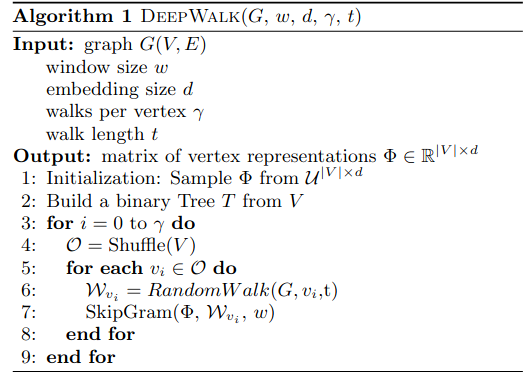
\includegraphics[width=10cm]{DeepWalkAlgorithm}
\centering
\end{figure}

The algorithm consists of two main components; first a random walk generator, and second, an update procedure. The random walk generator takes a graph $G$ and samples uniformly  a  random  vertex $v_{i}$ as  the  root  of  the  random walk $W_{v_{i}}$.  A walk samples uniformly from the neighbors of the last vertex visited until the maximum length $(t)$ is reached.  While we set the length of our random walks in the experiments to be fixed, there is no restriction for the random walks to be of the same length.  These walks could have restarts (i.e. a teleport probability of returning back to their root), but our preliminary results did not show any advantage of using restarts.  In practice, our implementation specifies a number of random walks $\gamma$ of length $t$ to start at each vertex. Lines $3-9$ in \textit{Algorithm 1} shows the core of our approach.The outer loop specifies the number of times,$gamma$, which we should start random walks at each vertex.  We think of each iteration as making a "pass" over the data and sample one walk per node during this pass.  At the start of each pass we generate a random ordering to traverse the vertices.  This is not strictly required, but is well known to speed up the convergence of stochastic gradient descent. In the inner loop, we iterate over all the vertices of the graph. For  each  vertex $v_{i}$ we  generate  a  random  walk $|W_{v_{i}}|=t$,  and then use it to update our representations(Line 7).  We use the \textit{SkipGram algorithm} to update these representations in accordance with our objective function.


\subsubsection*{Algorithm : DeepWalk}

\begin{figure}[h]
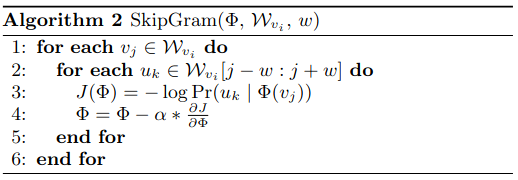
\includegraphics[width=8cm]{SkipGramAlgorithm}
\centering
\end{figure}


SkipGram algorithm is a popular technique used to learn word embeddings. It was introduced by Mikolov et. al. in their well-known paper on \textit{word2vec}. Given a corpus and a window size, \textit{SkipGram} aims to maximize the similarity of word embeddings’ of the words that occur in the same window. These windows are also called context in NLP. This idea is based on the assumption that: words that occurs in the same context tend to have same meanings. Therefore, their embeddings should be close to each other as well. To adapt SkipGram to networks, we need to determine what context corresponds to in the network world. This is where the random walks come into play. We can think of each walk produced in the previous step as a context or word window in a text. Thus, we can maximize the similarities of embeddings of nodes that occur on the same walks. In this sense, node sequences in networks correspond to word sequences in text. To learn the embeddings via \textit{SkipGram}, we first generate random vectors of dimension d for each node. Secondly, we iterate over the set of random walks and update the node embeddings by gradient descent to maximize the probability of the neighbors of a node, given the node itself. This can be achieved by the softmax function. When all of the walks are processed, we can either continue optimization with additional passes over the same walk set or generate new walks on the network.

\subsubsection*{Discussion}
Assume a network with node features and a node classification task. With traditional ML techniques, we can learn feature to label mappings by assuming that each instance is independent of each other. Clearly, this is an invalid assumption for network structured data. Thanks to DeepWalk, we can reflect neighborhood relations and local structures in the network to node representations. Since \textit{SkipGram} tries to maximize similarities of neighboring nodes, nodes are sharing information between each other. This means that we enrich our existing feature set with node embeddings that were learned in a self-supervised manner. Having learned new representations for nodes, we can now use classification models for our task. Yet, now we have got rid of an invalid assumption and introduced more information to our classifier. In the paper, authors have run extensive experiments to prove that \textit{DeepWalk} embeddings facilitate classification performance for several tasks. They have also run parameter sensitivity experiments to observe the influence of each parameter on the embedding quality.

\newpage

\section*{Node2Vec 2016}

Node2vec is an algorithmic framework for representational learning on graphs. Given any graph, it can learn continuous feature representations for the nodes, which can then be used for various downstream machine learning tasks. The \textit{node2vec} framework learns low-dimensional representations for nodes in a graph by optimizing a neighborhood preserving objective. The objective is flexible, and the algorithm accomodates for various definitions of network neighborhoods by simulating biased random walks. Specifically, it provides a way of balancing the exploration exploitation tradeoff that in turn leads to representations obeying a spectrum of equivalences from homophily to structural equivalence. 

\subsubsection*{Few consideration about Classic search strategies}

\begin{itemize}
\item Breadth-first Sampling (BFS): The neighborhood $N_{S}$ is restricted to nodes which are immediate neighbors of the source.
\item Depth-first Sampling (DFS) : The neighborhood consists of nodes sequentially sampled at increasing distances from thesource node.
\end{itemize}

We observe that BFS and DFS strategies play a key role in pro-ducing representations that reflect either of the above equivalences.In particular, the neighborhoods sampled by BFS lead to embeddings that correspond closely to structural equivalence. Intuitively, e note that in order to as certain structural equivalence,  it is often  sufficient  to  characterize  the  local  neighborhoods  accurately.For example, structural equivalence based on network roles such asbridges and hubs can be inferred just by observing the immediate neighborhoods of each node. By restricting search to nearby nodes,BFS achieves this characterization and obtains a microscopic view of the neighborhood of every node. Additionally, in BFS, nodes inthe sampled neighborhoods tend to repeat many times. This is also important as it reduces the variance in characterizing the distribution of $1-hop nodes$ with respect the source node. However, a very small portion of the graph is explored for any given $k$.The opposite is true for DFS which can explore larger parts ofthe network as it can move further away from the source nodeu(with sample size $k$ being fixed). In DFS, the sampled nodes more accurately reflect a macro-view of the neighborhood which is essential  in  inferring  communities  based  on  homophily.   However,the issue with DFS is that it is important to not only infer which node-to-node dependencies exist in a network, but also to characterize the exact nature of these dependencies.  This is hard given we have a constrain on the sample size and a large neighborhood to explore, resulting in high variance.  Secondly, moving to much greater depths leads to complex dependencies since a sampled nodemay be far from the source and potentially less representative.

\subsection*{Node2Vec Algorithm}

Building on the above observations, the authors design a flexible neighborhood sampling strategy which allows us to smoothly interpolatebetween BFS and DFS. they achieve this by developing a flexible biased random walk procedure that can explore neighborhoods in a BFS as well as DFS fashion.

\subsubsection*{Random Walks}
Formally, given a source node $u$, we simulate a random walk of fixed length $l$. Let $c_{i}$ denote the ith node in the walk, starting with $c_{0}=u$. Nodes $c_{i}$ are generated by the following distribution:

\begin{align*}
P(c_{i} | c_{i-1}=v) = \begin{cases} 
\pi_{vx} & if (v,x) \in E \\
0 & \text{otherwise}
\end{cases}
\end{align*}
Where $\pi_{vx}$ is the unnormalized transition probability between nodes v and x, and Z is the normalizing constant.

\subsubsection*{Search bias $\alpha$}

The simplest way to bias our random walks would be to sample the next node based on the static edge weights $w_{vx}$ i.e.,$\pi_{vx}=w_{vx}$.(In  case  of  un-weighted  graphs $w_{vx}= 1$.)   However,  this  does not  allow  us  to  account  for  the  network  structure  and  guide  our search procedure to explore different types of network neighborhoods. Additionally, unlike BFS and DFS which are extreme sampling paradigms suited for structural equivalence and homophily respectively,  our random walks should accommodate for the fact that these notions of equivalence are not competing or exclusive,and real-world networks commonly exhibit a mixture of both. We define a 2nd order random walk with two parameters $p$ and $q$ which guide the walk:  Consider a random walk that just travers edge$(t,v)$ and now resides at node $v$.  The walk now needs to decide on the next step so it evaluates the transition probabilities $\pi_{vx}$ on edges $(v,x)$ leading from $v$. 

\begin{align*}
\alpha_{pq}(t,x) = 
\begin{cases}
\frac{1}{p} & if d_{tx}=0 \\
1 & if d_{tx}=1 \\
\frac{1}{q} & if d_{tx}=2 \\
\end{cases}
\end{align*}

\begin{figure}[h]
\includegraphics[width=8cm]{node2vecPic}
\centering
\caption{Illustration of the random walk procedure in \textit{node2vec}.The walk just transitioned from $t$ to $v$ and is now evaluating its next step out of node $v$. Edge labels indicate search biases $\alpha$.}
\end{figure}

We set the un-normalized transition probability to $\pi_{vx}= \alpha_{pq}(t,x)w_{vx}$, where and $d_{tx}$ denotes the shortest path distance between nodes $t$ and $x$.Note that $d_{tx}$ must be one of $\{0,1,2\}$, and hence, the two parameters are necessary and sufficient to guide the walk. Intuitively, parameters $p$ and $q$ control how fast the walk exploresand leaves the neighborhood of starting node $u$. In particular, the parameters allow our search procedure to (approximately) interpolate between BFS and DFS and thereby reflect an affinity for different notions of node equivalences.
\\ \\
\textbf{Return parameter,p.}Parameter $p$ controls the likelihood of immediately revisiting a node in the walk.  Setting it to a high value $(>max(q,1))$ ensures that we are less likely to sample an already visited  node  in  the  following  two  steps  (unless  the  next  node  in the walk had no other neighbor).  This strategy encourages moderate exploration and avoids $2-hop$ redundancy in sampling.  On the other hand,  if $p$ is low $(<min(q,1))$,  it would lead the walk tobacktrack a step  and this would keep the walk “local” close to the starting node $u$.
\\ \\
\textbf{In-out parameter,q.}Parameter $q$ allows the search to differentiate between “inward” and “outward” nodes. if $q > 1$, the random walk is biased towards nodes close to node $t$. Such walks obtain a local view of the underlying graph with respect to the start node in the walk and approximate BFS behavior in the sense that our samples comprise of nodes within a small locality. In contrast, if $q <1$, the walk is more inclined to visit nodes which are further away from the node t.  Such behavior is reflective of DFS which encourages outward exploration.  However, an essential difference here is that we achieve DFS-like exploration within the random walk framework. Hence, the sampled nodes are not at strictly increasing distances from a given source node $u$, but in turn, we benefit from tractable preprocessing and superior sampling efficiency of random walks.  Note that by setting $\pi_{vx}$ to be a function of the preceeding node in the walk t, the random walks are $2^{nd}$ order Markovian.
\\ \\
\textbf{Benefits of random walks.} There are several benefits of random walks over pure BFS/DFS approaches. Random walks are computationally efficient in terms of both space and time requirements.The space complexity to store the immediate neighbors of everynode  in  the  graph  is $O(|E|)$.   For  $2^{nd}$ order  random  walks,  it  is helpful to store the interconnections between the neighbors of every node, which incurs a space complexity of $O(a^{2}|V|)$ where a is  the  average  degree  of  the  graph  and  is  usually  small  for  real-world networks.  The other key advantage of random walks over classic search-based sampling strategies is its time complexity.  Inparticular,  by imposing graph connectivity in the sample generation process, random walks provide a convenient mechanism to increase the effective sampling rate by reusing samples across different source nodes. By simulating a random walk of length $l > k$ we can generate k samples for $l-k$ nodes at once due to the Markovian nature of the random walk. Hence, our effective complexity is $O\left( \frac{l}{k(l-k)} \right)$


\begin{figure}[h]
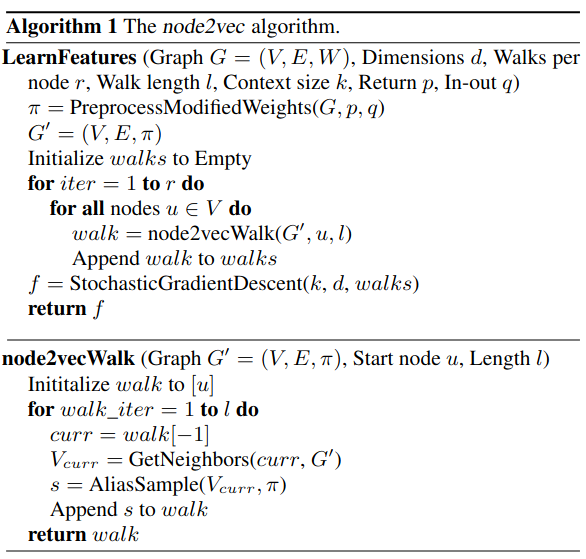
\includegraphics[width=8cm]{node2vecAlgorithm}
\centering
\end{figure}

The pseudocode for \textit{node2vec}.  In any random walk, there is an implicit bias due to the choice of the start node $u$. Since we learn representations for all nodes, we offset this bias by simulating $r$ random walks of fixed length $l$ starting from every node.  At every step of the walk, sampling is done based on the transition probabilities $\pi_{vx}$. The transition probabilities $\pi_{vx}$ for the $2^{nd}$ order Markov chain can be precomputed and hence, sampling of nodes while simulating the random walk can be done efficiently in $O(1)$ time using alias sampling.  The three phases of \textit{node2vec} ,i.e.,  preprocessing to compute transition probabilities,random  walk  simulations  and  optimization  using  SGD,  are  executed sequentially. Each phase is parallelizable and executed asynchronously, contributing to the overall scalability of \textit{node2vec}.

\newpage


\section*{Graph Concolutional Networks 2017 Kipf et al. }

GCN is a type of convolutional neural network that can work directly on graphs and take advantage of their structural information. It solves the problem of classifying nodes in a graph, where labels are only available for a small subset of nodes (semi-supervised learning).

\begin{figure}[h]
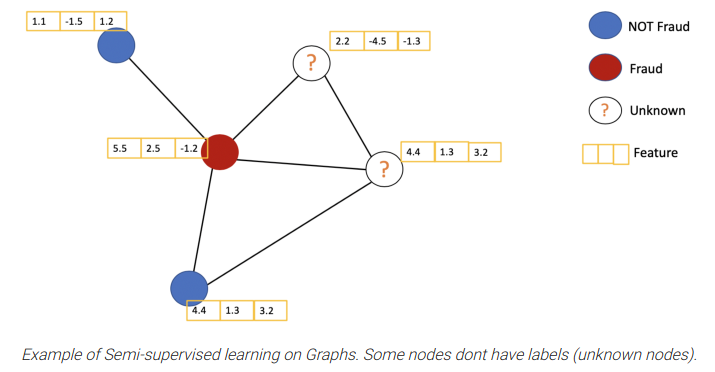
\includegraphics[width=10cm]{GCN_pic_1}
\centering
\end{figure}
GCNs themselves can be categorized into 2 major algorithms, Spatial Graph Convolutional Networks and Spectral Graph Convolutional Networks. The original idea behind Spectral GCN was inspired by signal/wave propagation. We can think of information propagation in Spectral GCN as signal propagation along the nodes. Spectral GCNs make use of the Eigen-decomposition of graph Laplacian matrix to implement this method of information propagation. To put it simply, the Eigen-decomposition helps us understand the graph structure, hence, classifying the nodes of the graphs. This is somewhat similar to the basic concept of Principal Component Analysis (PCA) and Linear Discriminant Analysis (LDA) where we use Eigen-decomposition to reduce dimensionality and perform clustering. 

\subsection*{GCNs Part I: Definitions}

Currently, most graph neural network models have a somewhat universal architecture in common. I will refer to these models as Graph Convolutional Networks (GCNs); convolutional, because filter parameters are typically shared over all locations in the graph (or a subset thereof as in Duvenaud et al., NIPS 2015).
\\ \\
For these models, the goal is then to learn a function of signals/features on a graph $G=(V,E)$ which takes as input:

\begin{itemize}
\item A feature description xi for every node i; summarized in a $N \times D$ feature matrix $X$ ($N$: number of nodes, $D$: number of input features)

\item A representative description of the graph structure in matrix form; typically in the form of an adjacency matrix $A$ (or some function thereof)
\end{itemize}
And produces a node-level output $Z$ (an $N \times F$ feature matrix, where $F$ is the number of output features per node). Graph-level outputs can be modeled by introducing some form of pooling operation (see, e.g. Duvenaud et al., NIPS 2015).
\\ \\
Every neural network layer can then be written as a non-linear function 

\begin{align*}
H^{l+1} = f(H^{l},A)
\end{align*}
With $H(0)=X$ and $H(L)=Z$ (or $z$ for graph-level outputs), $L$ being the number of layers. The specific models then differ only in how $f(\cdot,\cdot)$ is chosen and parameterized.


\subsection*{Fast Approximate Spectral Graph Convolutional Networks}

We consider a multi-layer Graph Convolutional Network (GCN) with the following layer-wise propagation rule:

\begin{align*}
H^{(l+1)} = \sigma( \tilde{D}^{-\frac{1}{2}} \tilde{A} \tilde{D}^{-\frac{1}{2}} H^{(l)} W^{(l)})
\end{align*}
Here, $\tilde{A} = A +I_{N}$ is the adjacency matrix of the undirected graph $G$ with added self-connections. $I_{N}$ is the identity matrix, $\tilde{D}_{ii} = \sum_{j} \tilde{A_{ij}}$ and $W^{(l)}$ is a layer-specific trainable weight matrix. $\sigma(\cdot)$ denotes an activation function, such as the $ReLU( \cdot ) = \max(0,\cdot)H^{l} \in \mathbb{R}^{N \times D}$ is the matrix of ac-tivations in the $l^{th}$ layer; $H^{0}=X$. In the following, we show that the form of this propagation rule can be motivated via a first-order approximation of localized spectral filters on graphs.




\subsubsection*{Spectral Graph Convolutions}
We consider spectral convolutions on graphs defined as the multiplication of a signal $x \in \mathbb{R}^{N}$ (as scalar for every node) with a filter $g_{\theta}=diag(\theta)$ parameterized by $\theta \in \mathbb{R}^{N}$  in the Fourier domain, i.e.:

\begin{align*}
g_{\theta^{'}} \approx \sum_{k=0}^{K}  \theta_{k}^{'} T_{k} ( \tilde{ \Lambda } )
\end{align*}
With a rescaled $\tilde{\Lambda} = \frac{2}{\lambda_{max}}\Lambda-I_{N}$. $\lambda_{max}$ denotes the largest eigenvalue of $L$. $\theta^{'} \ in \mathbb{R}^{K}$ is now avector of Chebyshev coefficients. The Chebyshev polynomials are recursively defined as $T_{k}(x)= 2xT_{k-1}(x)$, with $T_{0}(x)= 1$ and $T_{1}(x)=x$.  The reader is referred to \textit{Hammond et al.(2011)} for an in-depth discussion of this approximation.
\\ \\
Going back to our definition of a convolution of a signal $x$ with a filtering $\theta^{'}$, we now have:

\begin{align*}
g_{\theta^{'}} \star x \approx \sum_{k=0}^{K} \theta_{k}^{'} T_{k} ( \tilde{ L } )x
\end{align*}
With $\tilde{L} = \frac{2}{\lambda_{max}}L-I_{N}$; as can easily be verified by noticing that $(U\Lambda U^{T})^{k} = U\Lambda^{k} U^{T} $.  Note that this expression is now $K$-localized since it is a $K^{th}$-order polynomial in the Laplacian, i.e. it depends only on nodes that are at maximum $K$ steps away from the central node ($K^{th}$-order neighborhood). The complexity of evaluating $g_{\theta^{'}} \star x \approx \sum_{k=0}^{K} \theta_{k}^{'} T_{k} ( \tilde{ L } )x$ is $O(|E|)$, i.e. linear in the number of edges.  Defferrard et al.(2016) use this $K$-localized convolution to define a convolutional neural network on graphs.


\subsubsection*{Layer-Wise Linear Model}

A neural network model based on graph convolutions can therefore be built by stacking multiple convolutional layers, each layer followed by a point-wise non-linearity.  Now,imagine we limited the layer-wise convolution operation to $K= 1$, i.e. a function that is linear w.r.t. $L$ and therefore a linear function on the graph Laplacian spectrum. In this way, we can still recover a rich class of convolutional filter functions by stacking multiplesuch layers, but we are not limited to the explicit parameterization given by, e.g., the Chebyshev polynomials.  We intuitively expect that such a model can alleviate the problem of overfitting on local neighborhood structures for graphs with very wide node degree distributions, such as socialnetworks, citation networks, knowledge graphs and many other real-world graph datasets. Additionally, for a fixed computational budget, this layer-wise linear formulation allows us to build deeper models.
\\ \\
In this linear formulation of a GCN we further approximate $\lambda_{max} \approx 2$, as we can expect that neuralnetwork parameters will adapt to this change in scale during training.  Under these approximations

\begin{align*}
g_{\theta^{'}} \star x \approx \sum_{k=0}^{K} \theta_{k}^{'} T_{k} ( \tilde{ L } )x
\end{align*}
simplifies to:
\begin{align*}
g_{\theta^{'}} \star x \approx \theta_{0}^{'}x+\theta_{0}^{'}(L-I_{N})x = \theta_{0}^{'}x+\theta_{0}^{'} D^{-\frac{1}{2}}AD^{-\frac{1}{2}}x
\end{align*}
With two  free  parameters $\theta_{0}^{'}$ and $\theta_{1}^{'}$ .   The filter parameters  can  be shared over  the whole graph. Successive application of filters of this form then effectively convolve the $k^{th}$-order neighborhood ofa node, where $k$ is the number of successive filtering operations or convolutional layers in the neuralnetwork model.
\\ \\
In practice, it can be beneficial to constrain the number of parameters further to address overfittingand to minimize the number of operations (such as matrix multiplications) per layer. This leaves uswith the following expression:

\begin{align*}
g_{\theta^{'}} \star x \approx \theta \left(  I_{N}+D^{-\frac{1}{2}}AD^{-\frac{1}{2}} \right) x
\end{align*}
with  a  single  parameter $\theta = \theta_{0}^{'} = - \theta_{1}^{'}$. Note that $I_{N}+D^{-\frac{1}{2}}AD^{-\frac{1}{2}}$ now  has  eigenvalues  inthe range $[0,2]$. Repeated application of this operator can therefore lead to numerical instabilitiesand exploding/vanishing gradients when used in a deep neural network model.   To alleviate thisproblem, we introduce the following \textit{renormalization trick}: $I_{N}+D^{-\frac{1}{2}}AD^{-\frac{1}{2}}  \rightarrow D^{-\frac{1}{2}}\tilde{A} D^{-\frac{1}{2}}$, with $\tilde{A} = A +I_{N}$ and $\tilde{D}_{ii} = \sum_{i} \tilde{A}_{ij}$.
We can generalize this definition to a signal $X \in \mathbb{R}^{N \times C}$ with $C$ input channels (i.e. a $C$-dimensional feature vector for every node) and $F$ filters or feature maps as follows:

\begin{align*}
Z = \tilde{D}^{-\frac{1}{2}}\tilde{A}\tilde{D}^{-\frac{1}{2}}X \Theta
\end{align*}
Where $\Theta \in \mathbb{R}^{C \times F}$ is now a matrix of filter parameters and $Z \in \mathbb{R}^{C \times F}$. This the convolved signal matrix. This filtering operation has complexity $O(|E|FC)$, as $\tilde{A}X$ can be efficiently implemented as a product of a sparse matrix with a dense matrix.



\subsection*{GCNs Part II: A simple example}

As an example, let's consider the following very simple form of a layer-wise propagation rule:

\begin{align*}
f(H^{l},A) = \sigma (AH^{(l)}W^{(l)})
\end{align*}

where $W^{(l)}$ is a weight matrix for the l-th neural network layer and $\sigma(\cdot)$ is a non-linear activation function like the $ReLU$. Despite its simplicity this model is already quite powerful (we'll come to that in a moment).
\\ \\
But first, let us address two limitations of this simple model: multiplication with $A$ means that, for every node, we sum up all the feature vectors of all neighboring nodes but not the node itself (unless there are self-loops in the graph). We can "fix" this by enforcing self-loops in the graph: we simply add the identity matrix to $A$. 
\\ \\
The second major limitation is that $A$ is typically not normalized and therefore the multiplication with $A$ will completely change the scale of the feature vectors (we can understand that by looking at the eigenvalues of A). Normalizing $A$ such that all rows sum to one, i.e. $D^{-1}A$, where $D$ is the diagonal node degree matrix, gets rid of this problem. Multiplying with $D^{-1}A$ now corresponds to taking the average of neighboring node features. In practice, dynamics get more interesting when we use a symmetric normalization, i.e. $D^{-\frac{1}{2}}A^{-\frac{1}{2}}$ (as this no longer amounts to mere averaging of neighboring nodes). Combining these two tricks, we essentially arrive at the propagation rule introduced in Kipf et Welling (ICLR 2017):

\begin{align*}
f(H^{l},A) = \sigma (\hat{D}^{-\frac{1}{2}}\hat{A}^{-\frac{1}{2}}\hat{D}^{-\frac{1}{2}}H^{(l)}W^{(l)})
\end{align*}

with $\hat{A}=A+I$, where $I$ is the identity matrix and $\hat{D}$ is the diagonal node degree matrix of $\hat{A}$.

\subsection*{GCNs Part III: Embedding the karate club network}

\begin{figure}[h]
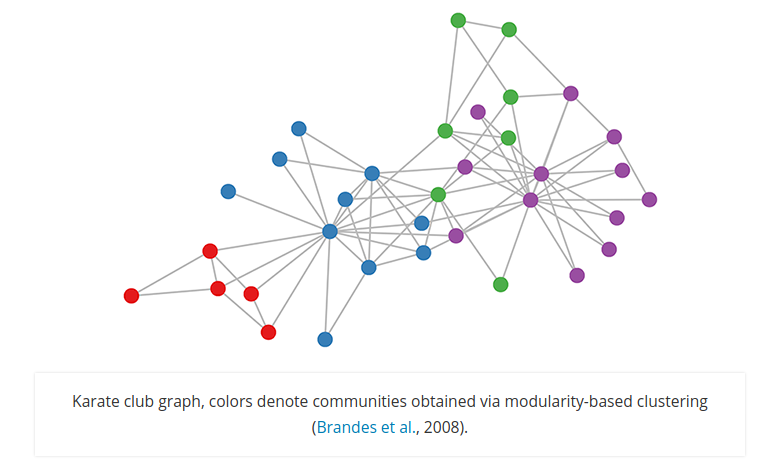
\includegraphics[width=8cm]{GCN-karate-club-network}
\centering
\end{figure}

Let's take a look at how our simple GCN model (see previous section or Kipf et Welling, ICLR 2017) works on a well-known graph dataset: Zachary's karate club network (see Figure above).
\\ \\
We take a 3-layer GCN with randomly initialized weights. Now, even before training the weights, we simply insert the adjacency matrix of the graph and $X=I$ (i.e. the identity matrix, as we don't have any node features) into the model. The 3-layer GCN now performs three propagation steps during the forward pass and effectively convolves the 3rd-order neighborhood of every node (all nodes up to 3 "hops" away). Remarkably, the model produces an embedding of these nodes that closely resembles the community-structure of the graph (see Figure below). Remember that we have initialized the weights completely at random and have not yet performed any training updates (so far)!

\begin{figure}[h]
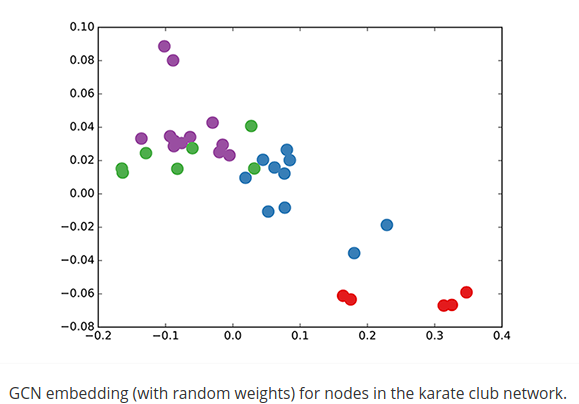
\includegraphics[width=8cm]{GCN-embeddings}
\centering
\end{figure}
This might seem somewhat surprising. A recent paper on a model called DeepWalk (Perozzi et al., KDD 2014) showed that they can learn a very similar embedding in a complicated unsupervised training procedure. How is it possible to get such an embedding more or less "for free" using our simple untrained GCN model?
\\ \\
We can shed some light on this by interpreting the GCN model as a generalized, differentiable version of the well-known Weisfeiler-Lehman algorithm on graphs. The (1-dimensional) Weisfeiler-Lehman algorithm works as follows3:
\\ \\
For all nodes $v_{i} \in G$:

\begin{itemize}
\item Get features $  h_{v_{j}}  $ of neighboring nodes $v_{j} $.
\item Update node feature $h_{v_{i}} \leftarrow hash(\sum_{j} h_{v_{j}})$, where $hash(\cdot)$ is (ideally) an injective hash function
\end{itemize}
Repeat for $k$ steps or until convergence.
\\ \\
In practice, the Weisfeiler-Lehman algorithm assigns a unique set of features for most graphs. This means that every node is assigned a feature that uniquely describes its role in the graph. Exceptions are highly regular graphs like grids, chains, etc. For most irregular graphs, this feature assignment can be used as a check for graph isomorphism (i.e. whether two graphs are identical, up to a permutation of the nodes).
\\ \\
Going back to our Graph Convolutional layer-wise propagation rule (now in vector form):

\begin{align*}
h_{v_{i}}^{(l+1)} = \sigma \left( \sum_{j} \frac{1}{c_{ij}} h_{v_{i}}^{(l)}W^{l}  \right)
\end{align*}
where $j$ indexes the neighboring nodes of $v_{i}$. $c_{ij}$ is a normalization constant for the edge $(v_{i},v_{j})$ which originates from using the symmetrically normalized adjacency matrix $D^{-\frac{1}{2}}AD^{-\frac{1}{2}}$ in our GCN model. We now see that this propagation rule can be interpreted as a differentiable and parameterized (with $W^{(l)}$) variant of the hash function used in the original Weisfeiler-Lehman algorithm. If we now choose an appropriate non-linearity and initialize the random weight matrix such that it is orthogonal (or e.g. using the initialization from Glorot et Bengio, AISTATS 2010), this update rule becomes stable in practice (also thanks to the normalization with cij). And we make the remarkable observation that we get meaningful smooth embeddings where we can interpret distance as (dis-)similarity of local graph structures!

\subsection*{GCNs Part IV: Semi-supervised learning}

Since everything in our model is differentiable and parameterized, we can add some labels, train the model and observe how the embeddings react. We can use the semi-supervised learning algorithm for GCNs introduced in Kipf et Welling (ICLR 2017). We simply label one node per class/community and start training for a couple of iterations.
Note that the model directly produces a 2-dimensional latent space which we can immediately visualize. We observe that the 3-layer GCN model manages to linearly separate the communities, given only one labeled example per class. This is a somewhat remarkable result, given that the model received no feature description of the nodes. At the same time, initial node features could be provided, which is exactly what we do in the experiments described in our paper (Kipf et Welling, ICLR 2017) to achieve state-of-the-art classification results on a number of graph datasets.

\newpage

\section*{Graph Attention Networks 2018}

GANs introduces an attention-based architecture to perform node classification of graph-structured data. The idea is to compute the hidden representations of each node in the graph, by attending over its neighbors, following a self-attention strategy. The attention architecture has several interesting properties: 

\begin{itemize}
\item[1] The operation is efficient, since it is parallelizable across node-neighbor pairs.
\item[2] It can be applied to graph nodes having different degrees by specifying arbitraryweights to the neighbors.
\item[3] The model is directly applicable toinductivelearning problems,including tasks where the model has to generalize to completely unseen graphs.
\end{itemize}

\subsection*{Towards a viable graph convolution}
Consider a graph of $n$ nodes, specified as a set of node features, $( \overrightarrow{h}_{1},\overrightarrow{h}_{2},...,\overrightarrow{h}_{n})$, and an adjacency matrix $A$, such that $A_{ij}=1$ if $i$ and $j$ are connected, and $0$ otherwise. A graph convolutional layer then computes a set of new node features, $(\overrightarrow{h}_{1}^{'},\overrightarrow{h}_{2}^{'},...,\overrightarrow{h}_{n}^{'})$, based on the input features as well as the graph structure. Every graph convolutional layer starts off with a shared node-wise feature transformation (in order to achieve a higher-level representation), specified by a weight matrix $W$. This transforms the feature vectors into $\overrightarrow{g}_{i}=W\overrightarrow{h}_{i}$. After this, the vectors $\overrightarrow{g}_{i}$ are typically recombined in some way at each node. In general, to satisfy the localisation property, we will define a graph convolutional operator as an aggregation of features across neighbourhoods; defining $N_{i}$ as the neighbourhood of node $i$ (typically consisting of all first-order neighbours of $i$, including $i$ itself), we can define the output features of node $i$ as:

\begin{align*}
\overrightarrow{h}_{i}^{'} = \sigma \left(  \sum_{j \in N_{i}} \alpha_{ij}\overrightarrow{g}_{i}^{'}  \right)
\end{align*}

Where $\sigma$ is an activation function, and $\alpha_{ij}$ specifies the weighting factor (importance) of node $j$’s features to node $i$. Most prior work defines $\alpha_{ij}$ explicitly (either based on the structural properties of the graph, or as a learnable weight); this requires compromising at least one other desirable property.
\\ \\
$\alpha_{ij}$ is implicitly defined, employing self-attention over the node features to do so. This choice was not without motivation, as self-attention has previously been shown to be self-sufficient for state-of-the-art-level results on machine translation, as demonstrated by the Transformer architecture (Vaswani et al., 2017 "attention is all you need").
\\ \\
Generally, we let $\alpha_{ij}$ be computed as a product of an attentional mechanism, $a: \mathbb{R}^{N} \times \mathbb{R}^{N} $, which computes un-normalised coefficients $e_{ij}$ across pairs of nodes $i$,$j$, based on their features:
\\ \\
We inject the graph structure by only allowing node $i$ to attend over nodes in its neighbourhood, $j \in N_{i}$. These coefficients are then typically normalised using the softmax function, in order to be comparable across different neighbourhoods:

\begin{align*}
\alpha_{ij} = \frac{exp(e_{ij})}{ \sum_{k \in N_{i} } exp(e_{ik})}
\end{align*}

The framework is agnostic to the choice of attentional mechanism $a$: in the experiments, the authors employed a simple single-layer neural network. The parameters of the mechanism are trained jointly with the rest of the network in an end-to-end fashion.

\subsection*{Regularisation}

To stabilise the learning process of self-attention, has been found multi-head attention to be very beneficial (as was the case in Vaswani et al., 2017). Namely, the operations of the layer are independently replicated $K$ times (each replica with different parameters), and outputs are featurewise aggregated (typically by concatenating or adding).

\begin{align*}
\overrightarrow{h}_{i}^{'} = \Bigg\|_{k=1}^{K} \sigma \left(  \sum_{j \in N_{i}} \alpha_{ij}^{k} W^{k}  \overrightarrow{h}_{j} \right) 
\end{align*}

where $\alpha_{ij}^{k}$ are the attention coefficients derived by the $k$-th replica, and $W^{k}$ the weight matrix specifying the linear transformation of the $k$-th replica.

\begin{figure}[h]
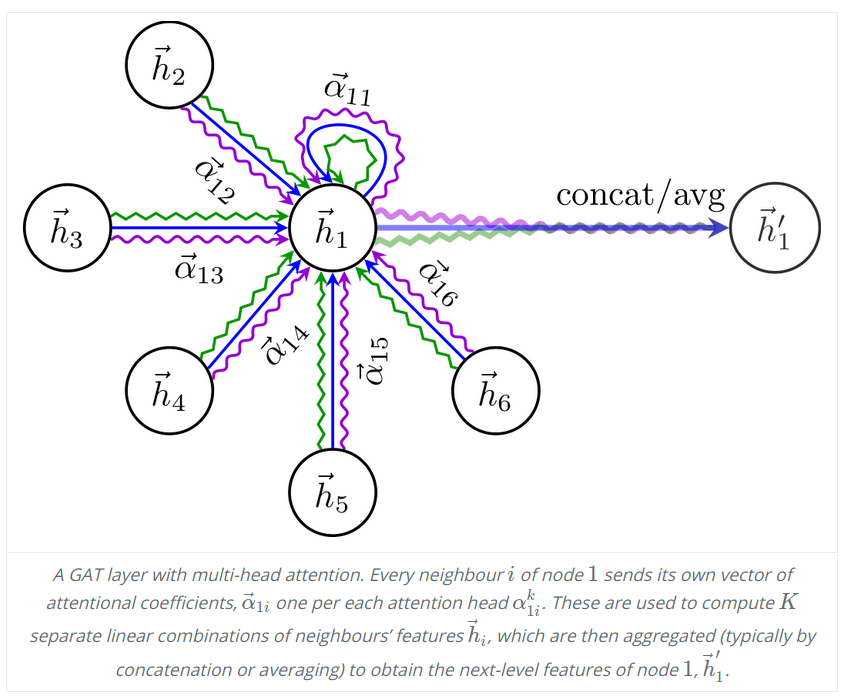
\includegraphics[width=8cm]{GAN-embeddings}
\centering
\end{figure}

Furthermore, has been found that applying dropout (Srivastava et al., 2014) to the attentional coefficients $\alpha_{ij}$ was a highly beneficial regulariser, especially for small training datasets. This effectively exposes nodes to stochastically sampled neighbourhoods during training, in a manner reminiscent of the (concurrently published) FastGCN method (Chen et al., 2018).

\subsection*{Conclusions}

Graph attention networks (GATs),is a convolution-style neural networks that operate on graph-structured data, leveraging masked self-attentional layers. The graph attentional layer utilised throughout these networks is computationally efficient (does not require costly matrix operations, and is parallelisable across all nodes in the graph), allows for (implicitly) assigning different importances to different nodes within a neighborhood while dealing with different sized neighborhoods, and does not depend on knowing the entire graph structure upfront—thus addressing many of the theoretical issues with approaches. Results, both within our work and the numerous subsequently published work, highlight the importance of such architectures towards building principled graph convolutional neural networks.


\newpage


\section*{GraphSAGE 2018}

Most node embedding models were based on spectral decomposition/matrix factorization methods. Matrix Factorization methods are inherently transductive. Simply put, a transductive method does not perform well on data it’s never seen before, i.e. these methods would expect the entire graph structure to be present on train time to generate node embeddings. If a new node is added to the graph at a later time, the model would have to be retrained. Conversely, an inductive approach would be one that can generalize to unseen data. An inductive approach to generating node embeddings also facilitates generalization across graphs with the same form of features: for example, one could train an embedding generator on protein-protein interaction graphs derived from a model organism, andthen easily produce node embeddings for data collected on new organisms using the trained model.
\\ \\
The inductive node embedding problem is especially difficult, compared to the transductive setting,because generalizing to unseen nodes requires “aligning” newly observed subgraphs to the node embeddings that the algorithm has already optimized on.  An inductive framework must learn to recognize structural properties of a node’s neighborhood that reveal both the node’s local role in thegraph, as well as its global position. In this work we both extend GCNs to the task of inductive unsupervised learning and propose a framework that generalizes the GCN approach touse trainable aggregation functions (beyond simple convolutions).
\\ \\
The authors propose a general framework, called GraphSAGE (\textit{SAmple and aggreGatE}), for inductive node embedding.  Unlike embedding approaches that are based on matrix factorization, the authors leverage node features (e.g., text attributes, node profile information, node degrees) in order to learn an embedding function that generalizes to unseen nodes. By incorporating node features in the learning algorithm, the model simultaneously learn the topological structure of each node’s neighborhood as well as the distribution of node features in the neighborhood.  While this work focus on feature-rich graphs (e.g., citation data with text attributes, biological data with functional/molecular markers), ourapproach can also make use of structural features that are present in all graphs (e.g., node degrees).Thus, our algorithm can also be applied to graphs without node features. Instead of training a distinct embedding vector for each node, this works propose to train a set of aggregator functions that learn to aggregate feature information from a node’s local neighborhood.

\begin{figure}[h]
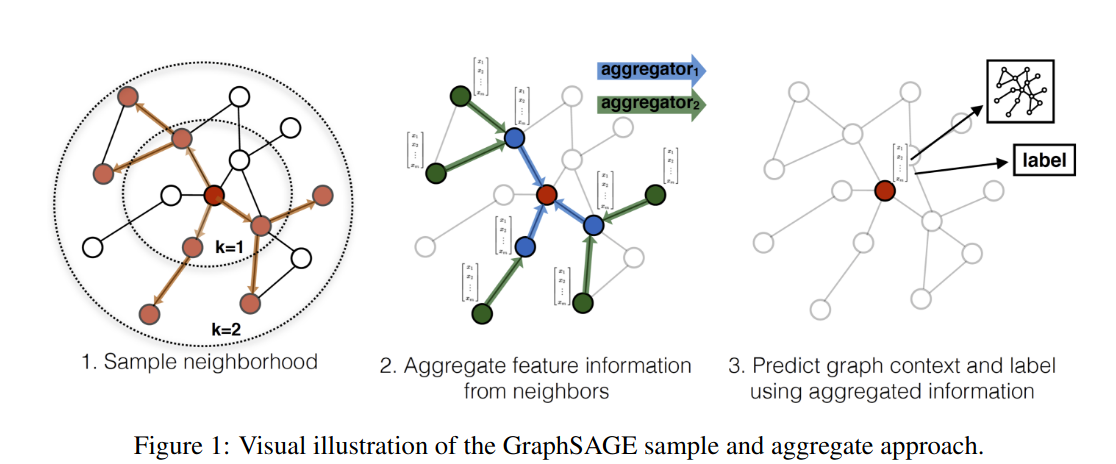
\includegraphics[width=10cm]{GraphSAGE-PIC-1}
\centering
\end{figure}
Each aggregator function aggregates information from a different number of hops, or search depth, away from a given node. At test, or inference time, the authors use the trained system to generate embeddings for entirely unseen nodes by applying the learned aggregation functions. Following previous work on generating node embeddings, thie framework design an unsupervised loss function that allows GraphSAGE to be trained without task-specific supervision. it also show that GraphSAGE can be trained in a fully supervised manner.

\subsection*{Proposed method: GraphSAGE}

The key idea behind this approach is that the model learn how to aggregate feature information from a node’s local neighborhood (e.g., the degrees or text attributes of nearby nodes).  the paper first describe the  GraphSAGE  embedding  generation  (i.e.,  forward  propagation)  algorithm,  which  generatesembeddings for nodes assuming that the GraphSAGE model parameters are already learned.Then is describes how the GraphSAGE model parameters can be learned using standard stochastic gradient descent and backpropagation techniques.

\subsubsection*{Embedding generation (i.e., forward propagation) algorith}


In this section, is described the embedding generation, or forward propagation algorithm, which assumes that the model has already been trained and that the parameters are fixed.  In particular, assume that we have learned the parameters of $K$ aggregator functions (denoted AGGREGATE $k,\forall k \in \{1,...,K\})$, which aggregate information from node neighbors, as well as a set of weight matrices $W^{k},\forall k \in \{1,...,K\}$, which are used to propagate information between differentlayers of the model or “search depths”. describes how we train these parameters.

\begin{figure}[h]
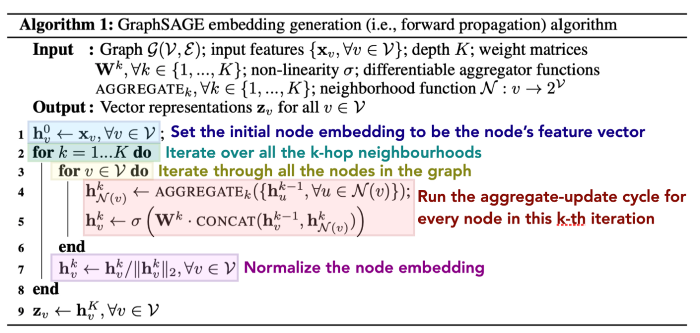
\includegraphics[width=10cm]{GraphSAGE-PIC-3}
\centering
\end{figure}
The intuition behind is that at each iteration, or search depth, nodes aggregate information from their local neighbors, and as this process iterates, nodes incrementally gain more and moreinformation from further reaches of the graph.
\\ \\
It describes the embedding generation process in the case where the entire graph,$G=(V,E)$, and features for all nodes $x_{v},\forall v \in V$, are provided as input. Each step in the outer loop of Algorithm proceeds as follows,where $k$ denotes the current step in the outer loop (or the depth of the search) and $h^{k}$ denotes a node’s representation at this step: First, each node $v \in V$ aggregates the representations of the nodes in its immediate neighborhood, $ \{h^{k-1}_{u},\forall u \in N(v)\}$, into a single vector $h^{k-1}_{N(v)}$ . Note that this aggregation step depends on the representations generated at the previous iteration of the outer loop $(i.e.,k-1)$,and the $k= 0$ (“base case”) representations are defined as the input node features. After aggregatingthe neighboring feature vectors, GraphSAGE then concatenates the node’s current representation,$h^{k-1}_{v}$, with the aggregated neighborhood vector,$h^{k-1}_{N(v)}$, and this concatenated vector is fed through a fully connected layer with non linear activation function $\sigma$, which transforms the representations to be used at the next step of the algorithm $(i.e.,h^{k}_{v},\forall v \in V)$. For notational convenience, we denotethe final representations output at depth $K$ as $z_{v} \equiv h^{K}_{v},\forall v \in V$. The aggregation of the neighbor representations can be done by a variety of aggregator architectures.

\subsection*{Relation to the Weisfeiler-Lehman Isomorphism Test.}

The GraphSAGE algorithm is conceptuallyinspired by a classic algorithm for testing graph isomorphism. If in (i) we set $K=|V|$,(ii) set the weight matrices as the identity, and (iii) use an appropriate hash function as an aggregator(with no non-linearity), then the algorithm is an instance of the Weisfeiler-Lehman (WL) isomorphismtest, also known as “naive vertex refinement”. If the set of representations $\{z_{v},\forall v \in V \} $ output by the algorithm for two subgraphs are identical then the WL test declares the two subgraphs to be isomorphic.  This test is known to fail in some cases, but is valid for a broad class of graphs. GraphSAGE is a continuous approximation to the WL test, where we replace the hash function with trainable neural network aggregators. Of course, we use GraphSAGE to generate useful node representations–not to test graph isomorphism. Nevertheless, the connection between GraphSAGE and the classic WL test provides theoretical context for our algorithm design to learn the topological structure of node neighborhoods.

\subsection*{Unsupervised loss function}

The authors train both unsupervised and supervised GraphSAGE models. The supervised setting follows a regular cross-entropy style prediction for a node classification task. The unsupervised case however tries to preserve graph structure by enforcing the following loss function:

\begin{figure}[h]
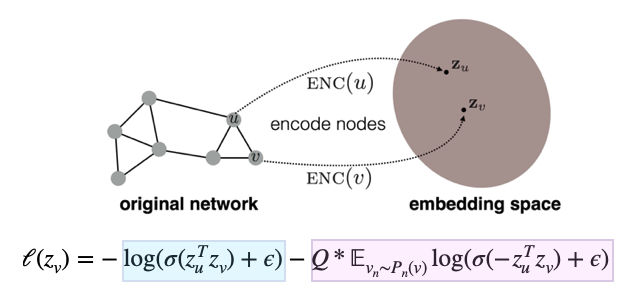
\includegraphics[width=10cm]{GraphSAGE-PIC-4}
\centering
\end{figure}
The blue portion of the loss function tries to enforce that if nodes u and v are close in the actual graph, then their node embeddings should be semantically similar. In the perfect scenario, we expect the inner product of $z_u$ and $z_v$ to be a large number. The sigmoid of this large number gets pushed towards $1$ and the $log(1) = 0$. The pink portion of the loss function tries to enforce the opposite! That is, if nodes $u$ and $v$ are actually far away in the actual graph, we expect their node embeddings to be different/opposite. In the perfect scenario, we expect the inner product of $z_{u}$ and $z_{v}$ to be a large negative number. This can be interpreted as, the embeddings $z_u$ and $z_v$ are so different that they are greater than 90 degrees apart. The product of two large negatives become a large positive number. The sigmoid of this large number gets pushed towards $1$ and the $log(1) = 0$. Since there are potentially more nodes $u$ that are far from our target node $v$ in the graph, we sample only a few negative nodes $u$ from the distribution of nodes far away from node $v: P_{n}(v)$. This ensures the loss function is balanced when training.
The addition of epsilon ensures we never take $log(0)$.

\newpage

%\section*{Graph Convolution on protein interaction}
%\begin{figure}[h]
%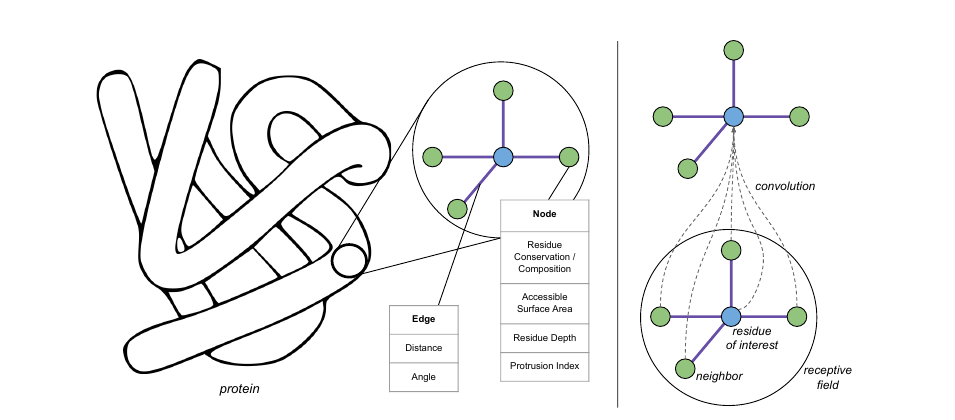
\includegraphics[width=10cm]{Protein-Interaction-Graph}
%\centering
%\caption{Graph convolution on protein structures. Left: Each residue in a protein is a node in a graph where theneighborhood of a node is the set of neighboring nodes in the protein structure; each node has features computedfrom its amino acid sequence and structure, and edges have features describing the relative distance and anglebetween residues. Right: Schematic description of the convolution operator which has as its receptive field a setof neighboring residues, and produces an activation which is associated with the center residue.}
%\end{figure}

\printbibliography

\end{document}

